\begin{exercice*}
    On considère le pavage ci-dessous.\\
    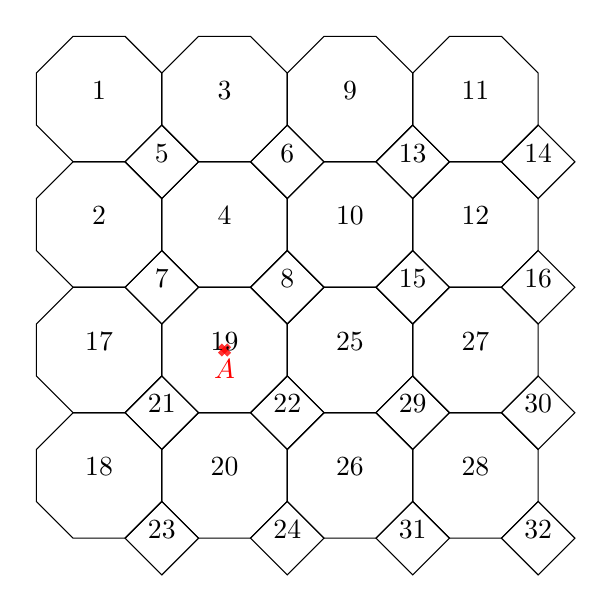
\begin{tikzpicture}[baseline,scale = 0.22]    
        \tikzset{
            point/.style={
            thick,
            draw,
            cross out,
            inner sep=0pt,
            minimum width=5pt,
            minimum height=5pt,
            },
        }
        \clip (-2.6213203435596424,-24.349120343559644) rectangle (29.470440687119282,7.742640687119283);
        \draw[color ={{red}},line width = 2,opacity = 0.8] (8.475933333333332,-10.597212989773693)--(9.009266666666667,-11.130546323107028);
        \draw[color ={{red}},line width = 2,opacity = 0.8] (8.475933333333332,-11.130546323107028)--(9.009266666666667,-10.597212989773693);
        \draw (8.7426,-10.86387965644036) node[below,color={red}] {$A$};        
        \draw[color={black}] (0,0)--(3,0)--(5.121320343559642,2.121320343559643)--(5.121320343559641,5.121320343559642)--(2.9999999999999982,7.242640687119283)--(-8.881784197001252e-16,7.242640687119282)--(-2.1213203435596424,5.121320343559639)--(-2.121320343559641,2.12132034355964)--cycle;
        \draw[color={black}] (3,0)--(0,0)--(-2.1213203435596424,-2.121320343559643)--(-2.121320343559642,-5.121320343559643)--(1.3322676295501878e-15,-7.242640687119286)--(3.0000000000000018,-7.242640687119285)--(5.121320343559644,-5.121320343559641)--(5.121320343559642,-2.121320343559641)--cycle;
        \draw[color={black}] (7.2426,0)--(10.2426,0)--(12.363920343559641,2.121320343559643)--(12.363920343559641,5.121320343559642)--(10.2426,7.242640687119283)--(7.2425999999999995,7.242640687119282)--(5.1212796564403575,5.121320343559639)--(5.121279656440359,2.12132034355964)--cycle;
        \draw[color={black}] (10.2426,0)--(7.2426,0)--(5.1212796564403575,-2.121320343559643)--(5.121279656440358,-5.121320343559643)--(7.242600000000001,-7.242640687119286)--(10.242600000000003,-7.242640687119285)--(12.363920343559645,-5.121320343559641)--(12.363920343559641,-2.121320343559641)--cycle;
        \draw[color={black}] (5.121320343559642,2.121320343559643)--(3,0)--(5.121320343559643,-2.121320343559642)--(7.242640687119285,1.0180718281354492e-15)--cycle;
        \draw[color={black}] (12.363920343559641,2.121320343559643)--(10.2426,0)--(12.363920343559643,-2.121320343559642)--(14.485240687119285,1.0180718281354492e-15)--cycle;
        \draw[color={black}] (5.121320343559642,-5.1212796564403575)--(3.0000000000000004,-7.2426)--(5.121320343559643,-9.363920343559641)--(7.242640687119285,-7.2425999999999995)--cycle;
        \draw[color={black}] (12.363920343559641,-5.1212796564403575)--(10.2426,-7.2426)--(12.363920343559643,-9.363920343559641)--(14.485240687119285,-7.2425999999999995)--cycle;
        \draw[color={black}] (14.4852,0)--(17.4852,0)--(19.60652034355964,2.1213203435596415)--(19.60652034355964,5.12132034355964)--(17.4852,7.242640687119282)--(14.485199999999999,7.242640687119281)--(12.363879656440357,5.1213203435596375)--(12.363879656440357,2.1213203435596375)--cycle;
        \draw[color={black}] (17.4852,0)--(14.4852,0)--(12.36387965644036,-2.1213203435596415)--(12.363879656440362,-5.121320343559639)--(14.485200000000006,-7.2426406871192786)--(17.485200000000003,-7.242640687119275)--(19.606520343559637,-5.121320343559632)--(19.60652034355963,-2.1213203435596375)--cycle;
        \draw[color={black}] (21.727800000000002,0)--(24.7278,0)--(26.84912034355964,2.1213203435596415)--(26.84912034355964,5.12132034355964)--(24.7278,7.242640687119282)--(21.7278,7.242640687119281)--(19.606479656440357,5.1213203435596375)--(19.606479656440357,2.1213203435596375)--cycle;
        \draw[color={black}] (24.7278,0)--(21.727800000000002,0)--(19.60647965644036,-2.1213203435596415)--(19.606479656440364,-5.121320343559639)--(21.727800000000006,-7.2426406871192786)--(24.727800000000002,-7.242640687119275)--(26.849120343559637,-5.121320343559632)--(26.84912034355963,-2.1213203435596375)--cycle;
        \draw[color={black}] (19.60652034355964,2.1213203435596415)--(17.4852,0)--(19.60652034355964,-2.121320343559642)--(21.727840687119283,1.2989340843532396e-16)--cycle;
        \draw[color={black}] (26.84912034355964,2.1213203435596415)--(24.7278,0)--(26.84912034355964,-2.121320343559642)--(28.970440687119282,1.2989340843532396e-16)--cycle;
        \draw[color={black}] (19.60652034355964,-5.121279656440359)--(17.4852,-7.2426)--(19.60652034355964,-9.363920343559641)--(21.727840687119283,-7.2426)--cycle;
        \draw[color={black}] (26.84912034355964,-5.121279656440359)--(24.7278,-7.2426)--(26.84912034355964,-9.363920343559641)--(28.970440687119282,-7.2426)--cycle;
        \draw[color={black}] (0,-14.4852)--(2.9999999999999964,-14.4852)--(5.121320343559637,-12.36387965644036)--(5.121320343559637,-9.363879656440364)--(2.9999999999999964,-7.242559312880724)--(-2.220446049250313e-16,-7.242559312880724)--(-2.12132034355964,-9.363879656440364)--(-2.12132034355964,-12.36387965644036)--cycle;
        \draw[color={black}] (2.9999999999999964,-14.4852)--(0,-14.4852)--(-2.1213203435596397,-16.60652034355964)--(-2.1213203435596393,-19.606520343559637)--(1.3322676295501878e-15,-21.727840687119276)--(2.999999999999997,-21.727840687119272)--(5.121320343559634,-19.60652034355963)--(5.1213203435596295,-16.606520343559634)--cycle;
        \draw[color={black}] (7.2426,-14.4852)--(10.242599999999996,-14.4852)--(12.363920343559638,-12.36387965644036)--(12.363920343559638,-9.363879656440364)--(10.242599999999996,-7.242559312880724)--(7.2426,-7.242559312880724)--(5.12127965644036,-9.363879656440364)--(5.12127965644036,-12.36387965644036)--cycle;
        \draw[color={black}] (10.242599999999996,-14.4852)--(7.2426,-14.4852)--(5.121279656440361,-16.60652034355964)--(5.121279656440361,-19.606520343559637)--(7.242600000000001,-21.727840687119276)--(10.242599999999998,-21.727840687119272)--(12.363920343559634,-19.60652034355963)--(12.36392034355963,-16.606520343559634)--cycle;
        \draw[color={black}] (5.121320343559637,-12.36387965644036)--(2.9999999999999964,-14.4852)--(5.121320343559637,-16.60652034355964)--(7.242640687119277,-14.4852)--cycle;
        \draw[color={black}] (12.363920343559638,-12.36387965644036)--(10.242599999999996,-14.4852)--(12.363920343559638,-16.60652034355964)--(14.485240687119276,-14.4852)--cycle;
        \draw[color={black}] (5.121320343559637,-19.60647965644036)--(2.999999999999997,-21.727800000000002)--(5.121320343559637,-23.84912034355964)--(7.242640687119277,-21.727800000000002)--cycle;
        \draw[color={black}] (12.363920343559638,-19.60647965644036)--(10.242599999999996,-21.727800000000002)--(12.363920343559638,-23.84912034355964)--(14.485240687119276,-21.727800000000002)--cycle;
        \draw[color={black}] (14.4852,-14.4852)--(17.4852,-14.4852)--(19.60652034355964,-12.363879656440359)--(19.60652034355964,-9.363879656440359)--(17.4852,-7.242559312880717)--(14.485199999999999,-7.242559312880718)--(12.363879656440357,-9.36387965644036)--(12.363879656440357,-12.36387965644036)--cycle;
        \draw[color={black}] (17.4852,-14.4852)--(14.4852,-14.4852)--(12.36387965644036,-16.60652034355964)--(12.36387965644036,-19.606520343559637)--(14.4852,-21.727840687119276)--(17.485199999999995,-21.727840687119272)--(19.60652034355963,-19.60652034355963)--(19.606520343559623,-16.606520343559637)--cycle;
        \draw[color={black}] (21.727800000000002,-14.4852)--(24.7278,-14.4852)--(26.84912034355964,-12.363879656440359)--(26.84912034355964,-9.363879656440359)--(24.7278,-7.242559312880717)--(21.7278,-7.242559312880718)--(19.606479656440357,-9.36387965644036)--(19.606479656440357,-12.36387965644036)--cycle;
        \draw[color={black}] (24.7278,-14.4852)--(21.727800000000002,-14.4852)--(19.60647965644036,-16.60652034355964)--(19.60647965644036,-19.606520343559637)--(21.727800000000002,-21.727840687119276)--(24.727799999999995,-21.727840687119272)--(26.84912034355963,-19.60652034355963)--(26.849120343559623,-16.606520343559637)--cycle;
        \draw[color={black}] (19.60652034355964,-12.363879656440359)--(17.4852,-14.4852)--(19.60652034355964,-16.606520343559644)--(21.727840687119283,-14.485200000000003)--cycle;
        \draw[color={black}] (26.84912034355964,-12.363879656440359)--(24.7278,-14.4852)--(26.84912034355964,-16.606520343559644)--(28.970440687119282,-14.485200000000003)--cycle;
        \draw[color={black}] (19.60652034355964,-19.60647965644036)--(17.4852,-21.727800000000002)--(19.60652034355964,-23.849120343559644)--(21.727840687119283,-21.727800000000002)--cycle;
        \draw[color={black}] (26.84912034355964,-19.60647965644036)--(24.7278,-21.727800000000002)--(26.84912034355964,-23.849120343559644)--(28.970440687119282,-21.727800000000002)--cycle;
        \draw [color={black},fill opacity = 1] (1.5,4.121320343559641) node[anchor = center,scale=1] {$1$};
        \draw [color={black},fill opacity = 1] (1.5000000000000004,-3.1213203435596424) node[anchor = center,scale=1] {$2$};
        \draw [color={black},fill opacity = 1] (8.742600000000001,4.121320343559641) node[anchor = center,scale=1] {$3$};
        \draw [color={black},fill opacity = 1] (8.742600000000001,-3.1213203435596424) node[anchor = center,scale=1] {$4$};
        \draw [color={black},fill opacity = 1] (5.121320343559642,0.5000000000000004) node[anchor = center,scale=1] {$5$};
        \draw [color={black},fill opacity = 1] (12.363920343559643,0.5000000000000004) node[anchor = center,scale=1] {$6$};
        \draw [color={black},fill opacity = 1] (5.121320343559642,-6.7425999999999995) node[anchor = center,scale=1] {$7$};
        \draw [color={black},fill opacity = 1] (12.363920343559643,-6.7425999999999995) node[anchor = center,scale=1] {$8$};
        \draw [color={black},fill opacity = 1] (15.985199999999999,4.12132034355964) node[anchor = center,scale=1] {$9$};
        \draw [color={black},fill opacity = 1] (15.985199999999999,-3.121320343559638) node[anchor = center,scale=1] {$10$};
        \draw [color={black},fill opacity = 1] (23.227799999999995,4.12132034355964) node[anchor = center,scale=1] {$11$};
        \draw [color={black},fill opacity = 1] (23.2278,-3.121320343559638) node[anchor = center,scale=1] {$12$};
        \draw [color={black},fill opacity = 1] (19.60652034355964,0.49999999999999994) node[anchor = center,scale=1] {$13$};
        \draw [color={black},fill opacity = 1] (26.849120343559637,0.49999999999999994) node[anchor = center,scale=1] {$14$};
        \draw [color={black},fill opacity = 1] (19.60652034355964,-6.7426) node[anchor = center,scale=1] {$15$};
        \draw [color={black},fill opacity = 1] (26.849120343559637,-6.7426) node[anchor = center,scale=1] {$16$};
        \draw [color={black},fill opacity = 1] (1.4999999999999982,-10.36387965644036) node[anchor = center,scale=1] {$17$};
        \draw [color={black},fill opacity = 1] (1.4999999999999973,-17.606520343559637) node[anchor = center,scale=1] {$18$};
        \draw [color={black},fill opacity = 1] (8.7426,-10.36387965644036) node[anchor = center,scale=1] {$19$};
        \draw [color={black},fill opacity = 1] (8.742599999999998,-17.606520343559637) node[anchor = center,scale=1] {$20$};
        \draw [color={black},fill opacity = 1] (5.121320343559637,-13.9852) node[anchor = center,scale=1] {$21$};
        \draw [color={black},fill opacity = 1] (12.363920343559638,-13.9852) node[anchor = center,scale=1] {$22$};
        \draw [color={black},fill opacity = 1] (5.121320343559637,-21.227800000000002) node[anchor = center,scale=1] {$23$};
        \draw [color={black},fill opacity = 1] (12.363920343559638,-21.227800000000002) node[anchor = center,scale=1] {$24$};
        \draw [color={black},fill opacity = 1] (15.985199999999999,-10.363879656440359) node[anchor = center,scale=1] {$25$};
        \draw [color={black},fill opacity = 1] (15.985199999999995,-17.606520343559637) node[anchor = center,scale=1] {$26$};
        \draw [color={black},fill opacity = 1] (23.227799999999995,-10.363879656440359) node[anchor = center,scale=1] {$27$};
        \draw [color={black},fill opacity = 1] (23.2278,-17.606520343559637) node[anchor = center,scale=1] {$28$};
        \draw [color={black},fill opacity = 1] (19.60652034355964,-13.985200000000003) node[anchor = center,scale=1] {$29$};
        \draw [color={black},fill opacity = 1] (26.849120343559637,-13.985200000000003) node[anchor = center,scale=1] {$30$};
        \draw [color={black},fill opacity = 1] (19.60652034355964,-21.227800000000002) node[anchor = center,scale=1] {$31$};
        \draw [color={black},fill opacity = 1] (26.849120343559637,-21.227800000000002) node[anchor = center,scale=1] {$32$};        
    \end{tikzpicture}\\        
    Soit la rotation de centre $A$ et d'angle \ang{90} dans le sens des aiguilles d'une montre.
    \begin{enumerate}
        \item Déterminer l'image de la figure $26$.
        \item Déterminer l'image de la figure $7$.
        \item Déterminer l'image de la figure $4$.
    \end{enumerate}
    \hrefMathalea{https://coopmaths.fr/mathalea.html?ex=3G12,s=1,s2=false,s3=5,s4=true,n=3,cd=1,i=0&v=l}
\end{exercice*}
\begin{corrige}
    %\setcounter{partie}{0} % Pour s'assurer que le compteur de \partie est à zéro dans les corrigés
    % \phantom{rrr}    
    On considère le pavage ci-dessous.\\
    \hspace*{-10mm}
    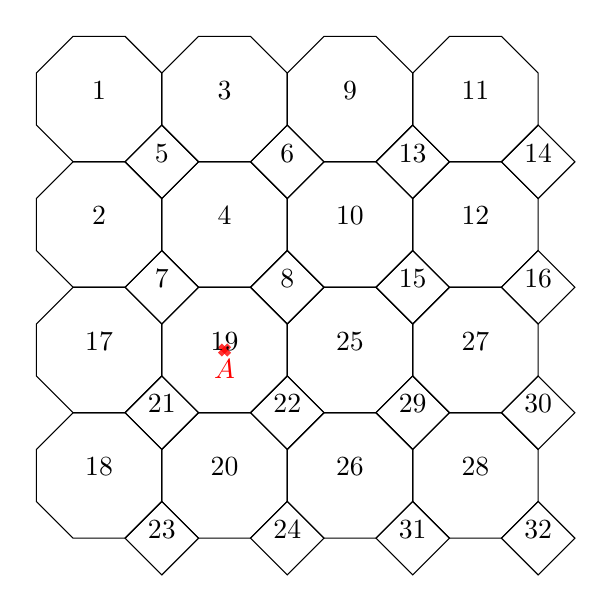
\begin{tikzpicture}[baseline,scale = 0.22]    
        \tikzset{
            point/.style={
            thick,
            draw,
            cross out,
            inner sep=0pt,
            minimum width=5pt,
            minimum height=5pt,
            },
        }
        \clip (-2.6213203435596424,-24.349120343559644) rectangle (29.470440687119282,7.742640687119283);
        \draw[color ={{red}},line width = 2,opacity = 0.8] (8.475933333333332,-10.597212989773693)--(9.009266666666667,-11.130546323107028);
        \draw[color ={{red}},line width = 2,opacity = 0.8] (8.475933333333332,-11.130546323107028)--(9.009266666666667,-10.597212989773693);
        \draw (8.7426,-10.86387965644036) node[below,color={red}] {$A$};        
        \draw[color={black}] (0,0)--(3,0)--(5.121320343559642,2.121320343559643)--(5.121320343559641,5.121320343559642)--(2.9999999999999982,7.242640687119283)--(-8.881784197001252e-16,7.242640687119282)--(-2.1213203435596424,5.121320343559639)--(-2.121320343559641,2.12132034355964)--cycle;
        \draw[color={black}] (3,0)--(0,0)--(-2.1213203435596424,-2.121320343559643)--(-2.121320343559642,-5.121320343559643)--(1.3322676295501878e-15,-7.242640687119286)--(3.0000000000000018,-7.242640687119285)--(5.121320343559644,-5.121320343559641)--(5.121320343559642,-2.121320343559641)--cycle;
        \draw[color={black}] (7.2426,0)--(10.2426,0)--(12.363920343559641,2.121320343559643)--(12.363920343559641,5.121320343559642)--(10.2426,7.242640687119283)--(7.2425999999999995,7.242640687119282)--(5.1212796564403575,5.121320343559639)--(5.121279656440359,2.12132034355964)--cycle;
        \draw[color={black}] (10.2426,0)--(7.2426,0)--(5.1212796564403575,-2.121320343559643)--(5.121279656440358,-5.121320343559643)--(7.242600000000001,-7.242640687119286)--(10.242600000000003,-7.242640687119285)--(12.363920343559645,-5.121320343559641)--(12.363920343559641,-2.121320343559641)--cycle;
        \draw[color={black}] (5.121320343559642,2.121320343559643)--(3,0)--(5.121320343559643,-2.121320343559642)--(7.242640687119285,1.0180718281354492e-15)--cycle;
        \draw[color={black}] (12.363920343559641,2.121320343559643)--(10.2426,0)--(12.363920343559643,-2.121320343559642)--(14.485240687119285,1.0180718281354492e-15)--cycle;
        \draw[color={black}] (5.121320343559642,-5.1212796564403575)--(3.0000000000000004,-7.2426)--(5.121320343559643,-9.363920343559641)--(7.242640687119285,-7.2425999999999995)--cycle;
        \draw[color={black}] (12.363920343559641,-5.1212796564403575)--(10.2426,-7.2426)--(12.363920343559643,-9.363920343559641)--(14.485240687119285,-7.2425999999999995)--cycle;
        \draw[color={black}] (14.4852,0)--(17.4852,0)--(19.60652034355964,2.1213203435596415)--(19.60652034355964,5.12132034355964)--(17.4852,7.242640687119282)--(14.485199999999999,7.242640687119281)--(12.363879656440357,5.1213203435596375)--(12.363879656440357,2.1213203435596375)--cycle;
        \draw[color={black}] (17.4852,0)--(14.4852,0)--(12.36387965644036,-2.1213203435596415)--(12.363879656440362,-5.121320343559639)--(14.485200000000006,-7.2426406871192786)--(17.485200000000003,-7.242640687119275)--(19.606520343559637,-5.121320343559632)--(19.60652034355963,-2.1213203435596375)--cycle;
        \draw[color={black}] (21.727800000000002,0)--(24.7278,0)--(26.84912034355964,2.1213203435596415)--(26.84912034355964,5.12132034355964)--(24.7278,7.242640687119282)--(21.7278,7.242640687119281)--(19.606479656440357,5.1213203435596375)--(19.606479656440357,2.1213203435596375)--cycle;
        \draw[color={black}] (24.7278,0)--(21.727800000000002,0)--(19.60647965644036,-2.1213203435596415)--(19.606479656440364,-5.121320343559639)--(21.727800000000006,-7.2426406871192786)--(24.727800000000002,-7.242640687119275)--(26.849120343559637,-5.121320343559632)--(26.84912034355963,-2.1213203435596375)--cycle;
        \draw[color={black}] (19.60652034355964,2.1213203435596415)--(17.4852,0)--(19.60652034355964,-2.121320343559642)--(21.727840687119283,1.2989340843532396e-16)--cycle;
        \draw[color={black}] (26.84912034355964,2.1213203435596415)--(24.7278,0)--(26.84912034355964,-2.121320343559642)--(28.970440687119282,1.2989340843532396e-16)--cycle;
        \draw[color={black}] (19.60652034355964,-5.121279656440359)--(17.4852,-7.2426)--(19.60652034355964,-9.363920343559641)--(21.727840687119283,-7.2426)--cycle;
        \draw[color={black}] (26.84912034355964,-5.121279656440359)--(24.7278,-7.2426)--(26.84912034355964,-9.363920343559641)--(28.970440687119282,-7.2426)--cycle;
        \draw[color={black}] (0,-14.4852)--(2.9999999999999964,-14.4852)--(5.121320343559637,-12.36387965644036)--(5.121320343559637,-9.363879656440364)--(2.9999999999999964,-7.242559312880724)--(-2.220446049250313e-16,-7.242559312880724)--(-2.12132034355964,-9.363879656440364)--(-2.12132034355964,-12.36387965644036)--cycle;
        \draw[color={black}] (2.9999999999999964,-14.4852)--(0,-14.4852)--(-2.1213203435596397,-16.60652034355964)--(-2.1213203435596393,-19.606520343559637)--(1.3322676295501878e-15,-21.727840687119276)--(2.999999999999997,-21.727840687119272)--(5.121320343559634,-19.60652034355963)--(5.1213203435596295,-16.606520343559634)--cycle;
        \draw[color={black}] (7.2426,-14.4852)--(10.242599999999996,-14.4852)--(12.363920343559638,-12.36387965644036)--(12.363920343559638,-9.363879656440364)--(10.242599999999996,-7.242559312880724)--(7.2426,-7.242559312880724)--(5.12127965644036,-9.363879656440364)--(5.12127965644036,-12.36387965644036)--cycle;
        \draw[color={black}] (10.242599999999996,-14.4852)--(7.2426,-14.4852)--(5.121279656440361,-16.60652034355964)--(5.121279656440361,-19.606520343559637)--(7.242600000000001,-21.727840687119276)--(10.242599999999998,-21.727840687119272)--(12.363920343559634,-19.60652034355963)--(12.36392034355963,-16.606520343559634)--cycle;
        \draw[color={black}] (5.121320343559637,-12.36387965644036)--(2.9999999999999964,-14.4852)--(5.121320343559637,-16.60652034355964)--(7.242640687119277,-14.4852)--cycle;
        \draw[color={black}] (12.363920343559638,-12.36387965644036)--(10.242599999999996,-14.4852)--(12.363920343559638,-16.60652034355964)--(14.485240687119276,-14.4852)--cycle;
        \draw[color={black}] (5.121320343559637,-19.60647965644036)--(2.999999999999997,-21.727800000000002)--(5.121320343559637,-23.84912034355964)--(7.242640687119277,-21.727800000000002)--cycle;
        \draw[color={black}] (12.363920343559638,-19.60647965644036)--(10.242599999999996,-21.727800000000002)--(12.363920343559638,-23.84912034355964)--(14.485240687119276,-21.727800000000002)--cycle;
        \draw[color={black}] (14.4852,-14.4852)--(17.4852,-14.4852)--(19.60652034355964,-12.363879656440359)--(19.60652034355964,-9.363879656440359)--(17.4852,-7.242559312880717)--(14.485199999999999,-7.242559312880718)--(12.363879656440357,-9.36387965644036)--(12.363879656440357,-12.36387965644036)--cycle;
        \draw[color={black}] (17.4852,-14.4852)--(14.4852,-14.4852)--(12.36387965644036,-16.60652034355964)--(12.36387965644036,-19.606520343559637)--(14.4852,-21.727840687119276)--(17.485199999999995,-21.727840687119272)--(19.60652034355963,-19.60652034355963)--(19.606520343559623,-16.606520343559637)--cycle;
        \draw[color={black}] (21.727800000000002,-14.4852)--(24.7278,-14.4852)--(26.84912034355964,-12.363879656440359)--(26.84912034355964,-9.363879656440359)--(24.7278,-7.242559312880717)--(21.7278,-7.242559312880718)--(19.606479656440357,-9.36387965644036)--(19.606479656440357,-12.36387965644036)--cycle;
        \draw[color={black}] (24.7278,-14.4852)--(21.727800000000002,-14.4852)--(19.60647965644036,-16.60652034355964)--(19.60647965644036,-19.606520343559637)--(21.727800000000002,-21.727840687119276)--(24.727799999999995,-21.727840687119272)--(26.84912034355963,-19.60652034355963)--(26.849120343559623,-16.606520343559637)--cycle;
        \draw[color={black}] (19.60652034355964,-12.363879656440359)--(17.4852,-14.4852)--(19.60652034355964,-16.606520343559644)--(21.727840687119283,-14.485200000000003)--cycle;
        \draw[color={black}] (26.84912034355964,-12.363879656440359)--(24.7278,-14.4852)--(26.84912034355964,-16.606520343559644)--(28.970440687119282,-14.485200000000003)--cycle;
        \draw[color={black}] (19.60652034355964,-19.60647965644036)--(17.4852,-21.727800000000002)--(19.60652034355964,-23.849120343559644)--(21.727840687119283,-21.727800000000002)--cycle;
        \draw[color={black}] (26.84912034355964,-19.60647965644036)--(24.7278,-21.727800000000002)--(26.84912034355964,-23.849120343559644)--(28.970440687119282,-21.727800000000002)--cycle;
        \draw [color={black},fill opacity = 1] (1.5,4.121320343559641) node[anchor = center,scale=1] {$1$};
        \draw [color={black},fill opacity = 1] (1.5000000000000004,-3.1213203435596424) node[anchor = center,scale=1] {$2$};
        \draw [color={black},fill opacity = 1] (8.742600000000001,4.121320343559641) node[anchor = center,scale=1] {$3$};
        \draw [color={black},fill opacity = 1] (8.742600000000001,-3.1213203435596424) node[anchor = center,scale=1] {$4$};
        \draw [color={black},fill opacity = 1] (5.121320343559642,0.5000000000000004) node[anchor = center,scale=1] {$5$};
        \draw [color={black},fill opacity = 1] (12.363920343559643,0.5000000000000004) node[anchor = center,scale=1] {$6$};
        \draw [color={black},fill opacity = 1] (5.121320343559642,-6.7425999999999995) node[anchor = center,scale=1] {$7$};
        \draw [color={black},fill opacity = 1] (12.363920343559643,-6.7425999999999995) node[anchor = center,scale=1] {$8$};
        \draw [color={black},fill opacity = 1] (15.985199999999999,4.12132034355964) node[anchor = center,scale=1] {$9$};
        \draw [color={black},fill opacity = 1] (15.985199999999999,-3.121320343559638) node[anchor = center,scale=1] {$10$};
        \draw [color={black},fill opacity = 1] (23.227799999999995,4.12132034355964) node[anchor = center,scale=1] {$11$};
        \draw [color={black},fill opacity = 1] (23.2278,-3.121320343559638) node[anchor = center,scale=1] {$12$};
        \draw [color={black},fill opacity = 1] (19.60652034355964,0.49999999999999994) node[anchor = center,scale=1] {$13$};
        \draw [color={black},fill opacity = 1] (26.849120343559637,0.49999999999999994) node[anchor = center,scale=1] {$14$};
        \draw [color={black},fill opacity = 1] (19.60652034355964,-6.7426) node[anchor = center,scale=1] {$15$};
        \draw [color={black},fill opacity = 1] (26.849120343559637,-6.7426) node[anchor = center,scale=1] {$16$};
        \draw [color={black},fill opacity = 1] (1.4999999999999982,-10.36387965644036) node[anchor = center,scale=1] {$17$};
        \draw [color={black},fill opacity = 1] (1.4999999999999973,-17.606520343559637) node[anchor = center,scale=1] {$18$};
        \draw [color={black},fill opacity = 1] (8.7426,-10.36387965644036) node[anchor = center,scale=1] {$19$};
        \draw [color={black},fill opacity = 1] (8.742599999999998,-17.606520343559637) node[anchor = center,scale=1] {$20$};
        \draw [color={black},fill opacity = 1] (5.121320343559637,-13.9852) node[anchor = center,scale=1] {$21$};
        \draw [color={black},fill opacity = 1] (12.363920343559638,-13.9852) node[anchor = center,scale=1] {$22$};
        \draw [color={black},fill opacity = 1] (5.121320343559637,-21.227800000000002) node[anchor = center,scale=1] {$23$};
        \draw [color={black},fill opacity = 1] (12.363920343559638,-21.227800000000002) node[anchor = center,scale=1] {$24$};
        \draw [color={black},fill opacity = 1] (15.985199999999999,-10.363879656440359) node[anchor = center,scale=1] {$25$};
        \draw [color={black},fill opacity = 1] (15.985199999999995,-17.606520343559637) node[anchor = center,scale=1] {$26$};
        \draw [color={black},fill opacity = 1] (23.227799999999995,-10.363879656440359) node[anchor = center,scale=1] {$27$};
        \draw [color={black},fill opacity = 1] (23.2278,-17.606520343559637) node[anchor = center,scale=1] {$28$};
        \draw [color={black},fill opacity = 1] (19.60652034355964,-13.985200000000003) node[anchor = center,scale=1] {$29$};
        \draw [color={black},fill opacity = 1] (26.849120343559637,-13.985200000000003) node[anchor = center,scale=1] {$30$};
        \draw [color={black},fill opacity = 1] (19.60652034355964,-21.227800000000002) node[anchor = center,scale=1] {$31$};
        \draw [color={black},fill opacity = 1] (26.849120343559637,-21.227800000000002) node[anchor = center,scale=1] {$32$};        
    \end{tikzpicture}\\        
    Soit la rotation de centre $A$ et d'angle \ang{90} dans le sens des aiguilles d'une montre.
    \begin{enumerate}
        \item Déterminer l'image de la figure $26$.\\
        {\red L'image de la figure $26$ est la figure $\boldsymbol{18}$.}
        \item Déterminer l'image de la figure $7$.\\
        {\red L'image de la figure $7$ est la figure $\boldsymbol{8}$.}        
        \item Déterminer l'image de la figure $4$.\\
        {\red L'image de la figure $4$ est la figure $\boldsymbol{25}$.}
    \end{enumerate}
\end{corrige}

